\documentclass[tikz,multi={tikzpicture},convert={outfile=images/ping-pong-2.png,density=1000}]{standalone}
\usepackage[build={latexoptions={-output-directory=latex/png}}]{standalone}
\usetikzlibrary{automata, positioning, arrows}
\usepackage{xcolor}
\newcommand{\StIdle}{\tiny\texttt{StIdle}}
\newcommand{\StBusy}{\tiny\texttt{StBusy}}
\newcommand{\StDone}{\tiny\texttt{StDone}}
\newcommand{\MsgPing}{\tiny\texttt{MsgPing}}
\newcommand{\MsgPong}{\tiny\texttt{MsgPong}}
\newcommand{\MsgDone}{\tiny\texttt{MsgDone}}
\newcommand{\StIdleX}{\tiny\texttt{StIdle2}}
\newcommand{\StBusyX}{\tiny\texttt{StBusy2}}
\newcommand{\StDoneX}{\tiny\texttt{StDone2}}
\newcommand{\MsgPingX}{\tiny\texttt{MsgPing2}}
\newcommand{\MsgPongX}{\tiny\texttt{MsgPong2}}
\newcommand{\MsgBusy}{\tiny\texttt{MsgBusy}}
\newcommand{\MsgDoneX}{\tiny\texttt{MsgDone2}}
\definecolor{mygreen}{rgb}{0.109804,0.698039,0.341176}
\definecolor{myblue}{rgb}{0.360784,0.423529,255}
\begin{document}
\tikzset{
    state/.style={
           rectangle,
           draw=white!40!black,
           minimum height=1em,
           inner sep=1pt,
           text centered
           },
    ->/.style={draw=white!40!black,-stealth}
}
\tikzstyle{every node}=[color=white!40!black,font=\tiny]
% Pipelined PingPong client
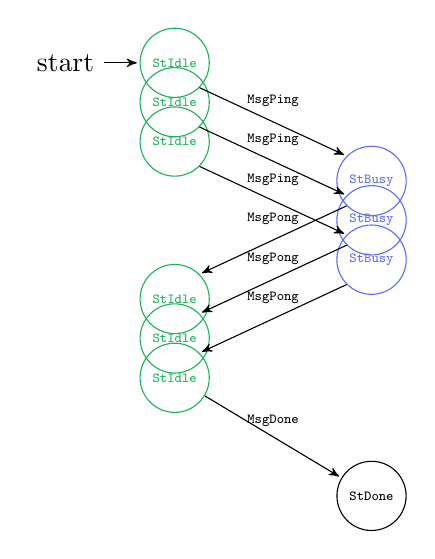
\begin{tikzpicture}[->,>=stealth',shorten >=1pt,auto,node distance=1.5cm]
  \node[state, mygreen, initial] (C0)  at (0, 0)      {\StIdle};
  \node[state, mygreen]          (C1)  at (0, -0.5)   {\StIdle};
  \node[state, mygreen]          (C2)  at (0, -1)     {\StIdle};
  \node[state, myblue]           (S0)  at (2.5, -1.5) {\StBusy};
  \node[state, myblue]           (S1)  at (2.5, -2)   {\StBusy};
  \node[state, myblue]           (S2)  at (2.5, -2.5) {\StBusy};
  \node[state, mygreen]          (C1') at (0, -3)     {\StIdle};
  \node[state, mygreen]          (C2') at (0, -3.5)   {\StIdle};
  \node[state, mygreen]          (C3)  at (0, -4)     {\StIdle};
  \node[state]                   (D)   at (2.5, -5.5) {\StDone};
  \draw[->] (C0.south east) -- node[above=0.07]{\MsgPing} (S0.north west);
  \draw[->] (C1.south east) -- node[above=0.07]{\MsgPing} (S1.north west);
  \draw[->] (C2.south east) -- node[above=0.07]{\MsgPing} (S2.north west);
  \draw[->] (S0.south west) -- node[above=0.07]{\MsgPong} (C1'.north east);
  \draw[->] (S1.south west) -- node[above=0.07]{\MsgPong} (C2'.north east);
  \draw[->] (S2.south west) -- node[above=0.07]{\MsgPong} (C3.north east);
  \draw[->] (C3) -- node[above]{\MsgDone} (D);
\end{tikzpicture}
\end{document}

